\chapter{Método e Planeamento}

\section{Metodologia de Desenvolvimento}

O desenvolvimento deste projeto segue uma abordagem iterativa e incremental, alinhada com metodologias adaptadas ao contexto académico e às necessidades específicas do AISIC LAB. Esta escolha fundamenta-se na necessidade de validação contínua com stakeholders e na natureza evolutiva dos requisitos de uma plataforma modular de anotação.

\subsection{Princípios Metodológicos}

A metodologia adotada assenta em três princípios fundamentais:

\begin{itemize}
    \item \textbf{Iterações Curtas}: Ciclos de desenvolvimento de duas semanas, permitindo feedback regular e ajustes frequentes
    \item \textbf{Validação Contínua}: Envolvimento regular dos stakeholders do AISIC LAB para validação de funcionalidades
    \item \textbf{Desenvolvimento Incremental}: Construção progressiva da plataforma, começando pelo módulo de disentanglement
\end{itemize}

\subsection{Organização do Trabalho}

O desenvolvimento está estruturado em sprints quinzenais, com os seguintes elementos:

\begin{itemize}
    \item \textbf{Planeamento}: Definição de objetivos e tarefas no início de cada sprint
    \item \textbf{Desenvolvimento}: Implementação das funcionalidades priorizadas
    \item \textbf{Revisão}: Avaliação do progresso e demonstração aos stakeholders
    \item \textbf{Retrospetiva}: Análise do processo e identificação de melhorias
\end{itemize}

\section{Planeamento e Cronograma}

O planeamento do projeto, representado na Figura~\ref{fig:gantt-chart}, está organizado em fases distintas que refletem a evolução da plataforma desde o protótipo inicial até à solução final.

\subsection{Fases do Projeto}

\subsubsection{Fase Inicial (Outubro - Dezembro 2024)}
Esta fase focou-se na validação de conceitos e estabelecimento de fundações:
\begin{itemize}
    \item Desenvolvimento do protótipo
    \item Validação da interface de anotação
    \item Levantamento tecnológico
    \item Documentação inicial
\end{itemize}

\subsubsection{MVP - Módulo Disentanglement (Dezembro 2024 - Janeiro 2025)}
Consolidação do protótipo existente:
\begin{itemize}
    \item Refinamento da interface frontend
    \item Testes de usabilidade
    \item Implementação de feedback inicial
    \item Validação com utilizadores piloto
\end{itemize}

\subsubsection{Infraestrutura Base (Janeiro - Março 2025)}
Estabelecimento da arquitetura modular:
\begin{itemize}
    \item Setup do ambiente de desenvolvimento
    \item Migração do backend para Python
    \item Implementação da arquitetura modular
    \item Sistema de autenticação
\end{itemize}

\subsubsection{Plataforma Core (Março - Maio 2025)}
Desenvolvimento das funcionalidades principais:
\begin{itemize}
    \item Framework para múltiplos módulos
    \item Sistema de gestão de datasets
    \item API base para integração
    \item Interface de administração
\end{itemize}

\subsubsection{Finalização (Maio - Junho 2025)}
Preparação para disponibilização:
\begin{itemize}
    \item Testes extensivos
    \item Validação com utilizadores
    \item Documentação técnica
    \item Deployment em produção
\end{itemize}

\section{Análise Crítica ao Planeamento}

\subsection{Progresso Atual}

O desenvolvimento inicial centrou-se na validação do conceito através de um protótipo funcional, que permitiu:

\begin{itemize}
    \item Validar a viabilidade técnica da solução proposta
    \item Confirmar a adequação da interface para tarefas de disentanglement
    \item Identificar pontos de melhoria no fluxo de trabalho
    \item Recolher feedback inicial dos utilizadores
\end{itemize}

\subsection{Desafios e Ajustes}

\subsubsection{Desafios Técnicos}
\begin{itemize}
    \item Complexidade na implementação da arquitetura modular
    \item Migração do backend para Python mantendo funcionalidade
    \item Otimização do processamento para datasets extensos
\end{itemize}

\subsubsection{Desafios Operacionais}
\begin{itemize}
    \item Balanceamento entre funcionalidades desejadas e prazos
    \item Adaptação a requisitos emergentes do AISIC LAB
\end{itemize}

\subsection{Adaptações ao Plano Original}

Com base na experiência do desenvolvimento inicial, foram identificados ajustes necessários:

\begin{itemize}
    \item Maior ênfase em testes de usabilidade
    \item Simplificação inicial de algumas funcionalidades
    \item Foco aumentado na documentação técnica
    \item Integração contínua de feedback dos utilizadores
\end{itemize}

\begin{landscape}
    \begin{figure}[p]
        \centering
        \makebox[\textwidth][c]{%
            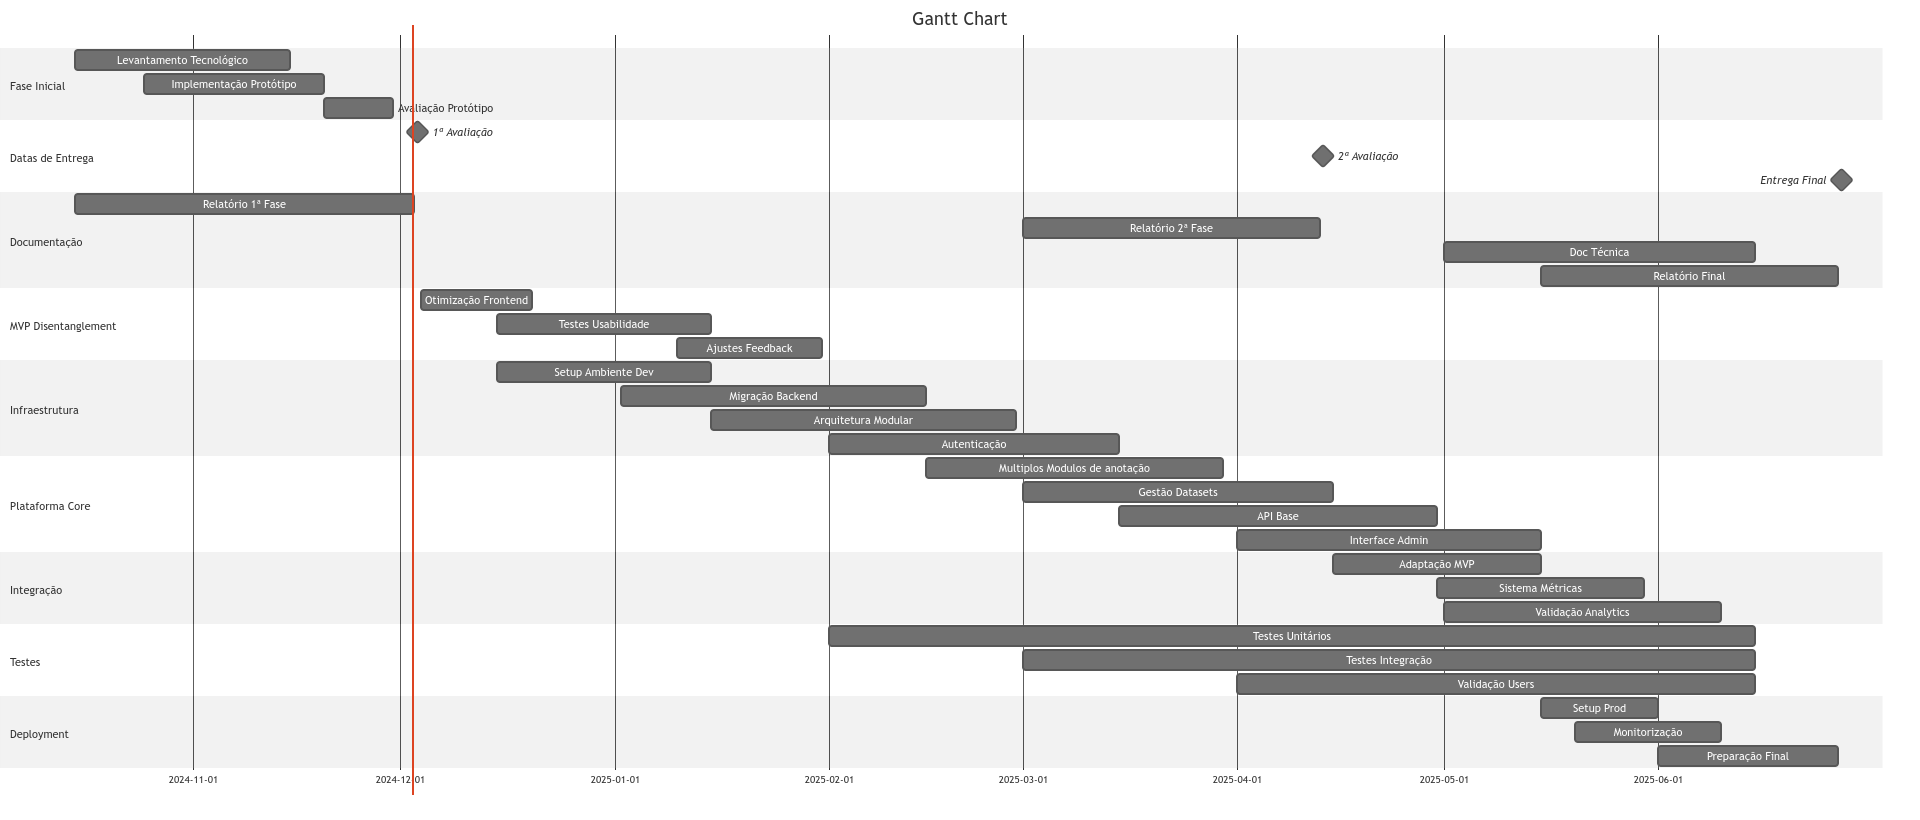
\includegraphics[width=0.98666\paperheight, angle=0, keepaspectratio]{images/Gant.drawio.png}
        }
        \caption{Cronograma detalhado do projeto (Gantt Chart)}
        \label{fig:gantt-chart}
    \end{figure}
\end{landscape}
